\documentclass{ieeeaccess}
\usepackage{cite}
\usepackage{amssymb,amsfonts}
\usepackage{algorithmic}
\usepackage{graphicx}
\usepackage{textcomp}
\usepackage{changes}
\usepackage{subcaption}
\usepackage{xcolor}
\usepackage{color, soul}
\usepackage{amsmath}
\def\BibTeX{{\rm B\kern-.05em{\sc i\kern-.025em b}\kern-.08em
    T\kern-.1667em\lower.7ex\hbox{E}\kern-.125emX}}
\graphicspath{{image/}}
\makeatletter
\def\endthebibliography{%
	\def\@noitemerr{\@latex@warning{Empty `thebibliography' environment}}%

}
\makeatother


\begin{document}
\history{Date of publication xxxx 00, 0000, date of current version xxxx 00, 0000.}
\doi{10.1109/ACCESS.2017.DOI}

\title{WSNNet: Bidirectional LSTM with Residual Attention for Indoor Localization of Wireless Sensor Network}
\author{\uppercase{HYUNGTAE LIM}\authorrefmark{1}, \IEEEmembership{Student Member, IEEE},
	\uppercase{CHANGGYU PARK}\authorrefmark{1}, \IEEEmembership{Student Member, IEEE},
	\uppercase{ and Hyun Myung}.\authorrefmark{1},
	\IEEEmembership{Senior Member, IEEE}}
\address[1]{Urban Robotics Laboratory, Korea Advanced Institute of Science and Technology, Daejeon 34141, South Korea.}

\tfootnote{This material is based upon work supported by the Ministry of Trade, Industry \& Energy(MOTIE, Korea) under Industrial Technology Innovation Program. No.10067202, 'Development of Disaster Response Robot System for Lifesaving and Supporting Fire Fighters at Complex Disaster Environment'.}

\markboth
{Author \headeretal: Preparation of Papers for IEEE TRANSACTIONS and JOURNALS}
{Author \headeretal: Preparation of Papers for IEEE TRANSACTIONS and JOURNALS}

\corresp{Corresponding author: Hyun Myung (hmyung@kaist.ac.kr).}

\begin{abstract}
	

As verified experimentally, this new proposal represents a significant improvement in accuracy, computation time, and robustness against outliers.

\end{abstract}

\begin{keywords}
Enter key words or phrases in alphabetical 
order, separated by commas. For a list of suggested keywords, send a blank 
e-mail to keywords@ieee.org or visit \underline
{http://www.ieee.org/organizations/pubs/ani\_prod/keywrd98.txt}
\end{keywords}

\titlepgskip=-15pt

\maketitle

\section{Introduction}
\label{sec:introduction}

\PARstart{S}{imultaneous} Localization and Mapping(SLAM) is widely used in autonomous vehicles, drones, intelligence field robots, and mobile phone applications. Thus, according to the smart city development plan, several technologies are required in such a way that the demand and the necessity of SLAM increase together. Various kinds of sensors are utilized to SLAM, such as GPS, LiDAR, ultrasonic-based sensor, camera and distance sensor. Especially, trilateration algorithm has been widely incorporated into robotics fields, especially utilized in the indoor environment to estimate the position of an object by distance measurements obtained from range sensors such as UWB, ultrasonic, laser-based beacon sensors \cite{thomas2005revisiting, cho2010mobile,raghavan2010accurate} due to the convenience of trilateration that estimates the position of a receiver of range sensors if one only knows range measurement. For that reasons, range-only Simultaneous Localization and Mapping(RO-SLAM) methods are utilized popularly, which not only estimate the position of the receiver of range sensors, but also localize the position of range sensors regarded as features on a map, and studies have been conducted continuously in terms of probability-based approach\cite{blanco2008pure,blanco2008efficient,fabresse2013undelayed, shetty2018particle}.

%확률적으로 접근했따

In the meantime, as deep learning age has come\cite{lecun2015deep}, various kinds of deep neural architectures have been proposed for many tasks related to robotics field, such as detection\cite{lenz2015deep,cai2016unified, smith2018object}, navigation\cite{zhu2017target, hamandi2018deepmotion}, pose estimation\cite{walch2017image}, and so on. Especially, recurrent neural networks (RNNs), originated from Natural Language Process(NLP) area\cite{elman1990finding}, have been shown to achieve better performance in case of dealing with time variant information, thereby RNNs are widely utilized such as not only speech recognition, but also pose estimation and localization\cite{walch2017image, gladh2016deep, wang2017deepvo, kendall2015posenet, turan2018deep}. 

In this paper, we propose a deep learning-based SLAM method by multimodal stacked bidirectional Long Short-Term Memory(multimodal stacked Bi-LSTM) for more accurate localization of the robot. Using deep learning, our structure directly learns the end-to-end mapping between range measurements and robot position. This operation non-linearly maps the relationship not only considering the long-range dependence of sequential distance data by the LSTM, but also using the correlation of the backward information and the forward information of the sequence of each time step by virtue of its bidirectional architecture. \textcolor{red}{Existing RO SLAM needs calibration before filtering, and then, range measurement undergoes outlier rejection, prediction and correction processes are needed.	Furthermorme, it uses low dimensional data to perform localization, there is a disadvantage that estimation is difficult even if the value deviates slightly from the model.} \textcolor{green}{Therefore, we solve this complex algorithm with end-to-end based deep learning. This system overview is shown in the figure below.}

Various kinds of sensors have been utilized to localize a object using range measurement sensors, such as GPS, ultrasonic-based sensors. ultra-wideband(UWB) sensors. However, almost distance measured by range measurement sensors are based on Time of Flight(TOF), Time of Arriaval(TOA)\cite{jung2011indoor}, or Time of Differential Arrival(TDOA) in such a way as to consist of the 1-D data composed by the distance between landmarks and robot. This is the main issue dealing with range measurments, called \textit{rank-dificiency} problems. Besides, only mangitudes could represent the range measurement, deflection, reflection, and refraction and ic  Because range measurements consist of    


In contrast to other SLAM, RO SLAM suffer from “rank deficiency problem”, which means range measurement is 1D data so it is too deficient to describe position or orientation as you guys knows, it only has magnitude. As this figure shown, in 3D, posiibility of location of sensor is distributed over sphere / since range measurement doesn’t contain direction information!
To solve this problem, various type of RO SLAM has been studied. RO SLAM is generally divided into two approaches; PF RO SLAM and KF based RO SLAM

%실험했다 얘기할 떄
. We also provide statistical analysis from simulations demonstrating that
our new approach can cope with highly noisy sensors and
reduces in one order of magnitude the average errors of the
method proposed

The rest of the paper is organized as follows. Section 2 describes relevant localization methods. Section 3 introduces
principals of neural networks. The experiments by which
these methods will be compared are given in Section 4. The
results will be discussed in Section 5, and concluding comments will be made in Section 6

fixed or calculated during initialization stage [7].
For range-based methods, the distance information can
be obtained by analyzing time of arrival (TOA), time
difference of arrival (TDOA), angle of arrival (AOA), or
received signal strength indicators (RSSI) [8]. TOA algorithm
calculates the distance on the basis of known transmission time and signal propagation speed. It requires highresolution clocks to be installed at sensor nodes. In case of
AOA algorithm, the sensor node needs several narrow beam
receivers or an antenna array to determine the direction of
the received signal. TDOA uses two transmission signals
of different propagation speeds. Therefore, it requires two
different transmitters and receivers on each node. The above
range-based localization techniques have little practical use
in WSNs due to the necessity of additional hardware, which
increases cost, size, and energy consumption of sensor nodes.
RSSI algorithms estimate the node-to-node distances by
using a signal propagation model. However, for real world

ference nodes.
Currently, there is a considerable research interest in
developing fingerprint localization methods based on artificial neural networks (ANNs) [10]. An important advantage
of this approach is that the ANN enables accurate recognition of node location in case of noisy RSSI measurements.
When using ANNs, the detailed information about indoor
environment and locations of the reference nodes is not
necessary. ANN interpolates the data collected in the fingerprint database to approximate a mapping between the
multidimensional fingerprints space and the coordinates of
nodes. In training phase, the collected RSSI vectors are used
to tune weights of connections between neurons in the ANN.
Although training can be time-consuming, the localization
process is much faster than analytical estimation of the node
location.
In this paper a method is proposed that improves localization accuracy of the ANN-based fingerprinting. According
to the introduced method, the entire localization area is
divided into regions by clustering the fingerprint database.
A separate ANN is trained for each region by using only
those fingerprints that belong to this region (cluster). During
clustering, a prototype RSSI vector is determined for each
region. When localization process starts, those prototypes are
selected that are most similar to the vector of current RSSI
measurements. The ANNs that correspond to the selected
prototypes are used to estimate the node coordinates. Final
estimation of the location is obtained by fusion of the
coordinates delivered by ANNs. Further improvement of the
localization accuracy as well as speedup of learning process
was achieved by employing fully connected neural networks

We propose a novel range-free localization algorithm
for wireless sensor networks that is robust against the anisotropic
signal attenuation

++++++

\begin{figure}[h]
	\centering
	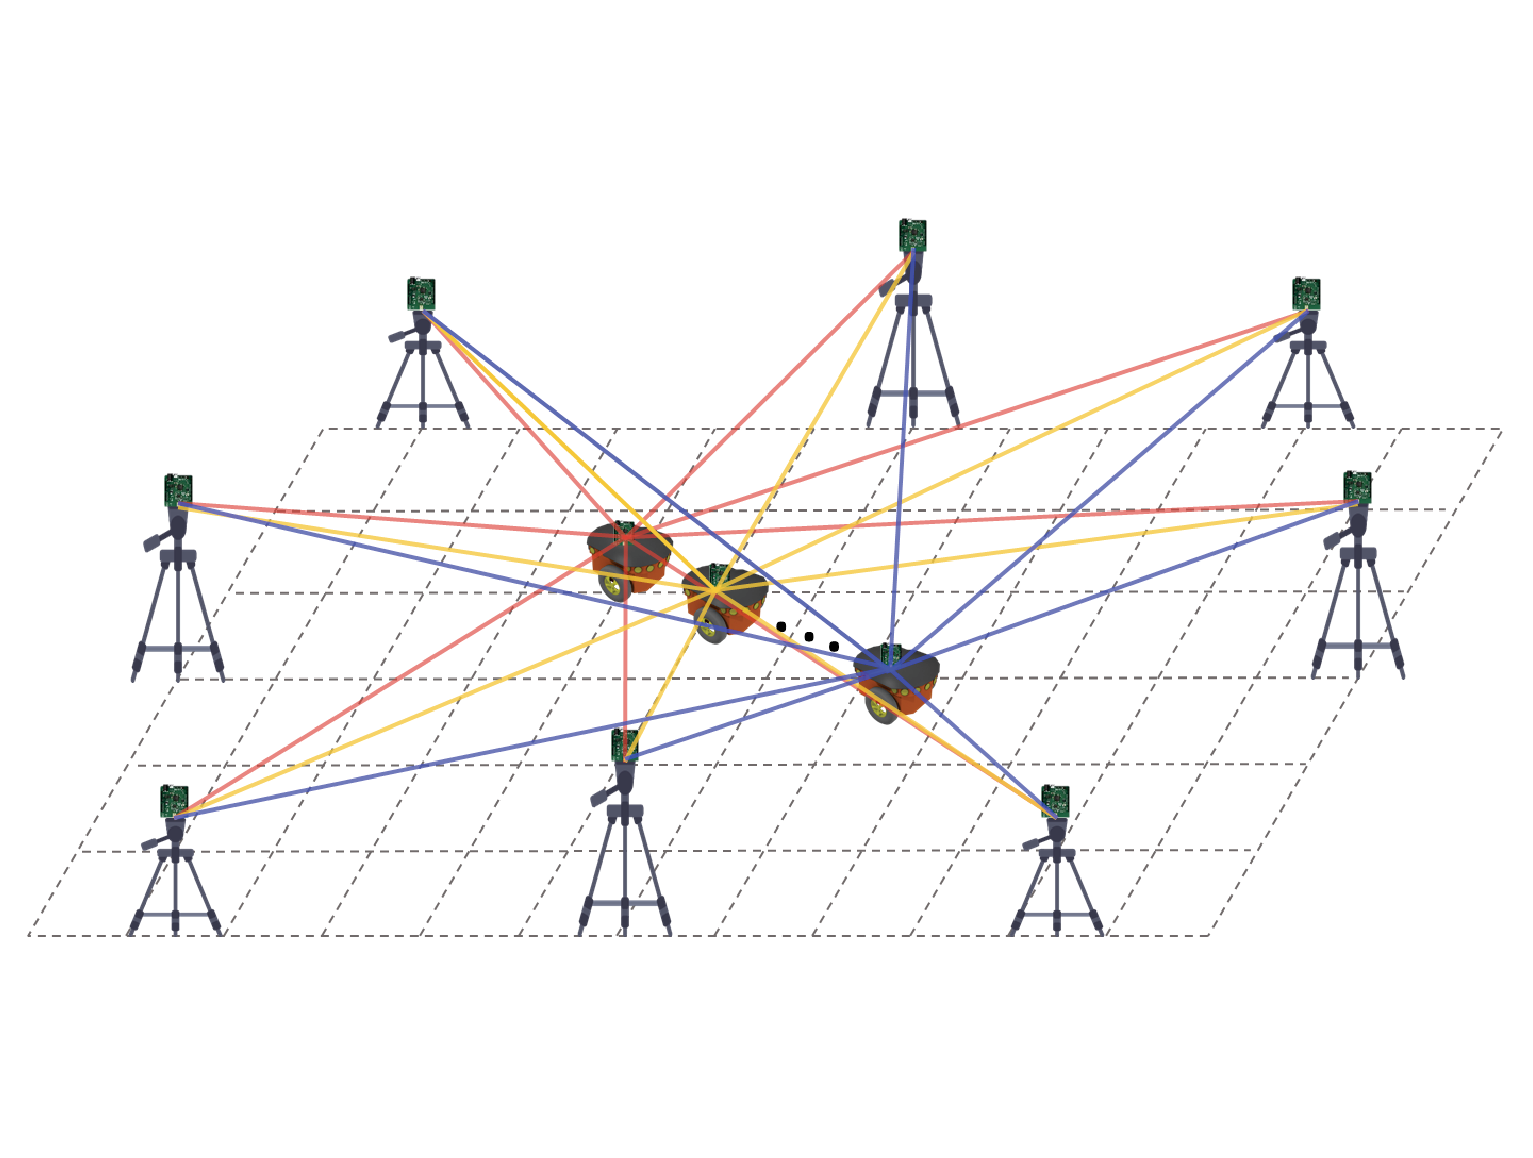
\includegraphics[width=.5\textwidth]{image/Access_overview_figure_1}
	\caption{Figures from experiment (a)The anchor and tag nodes (b)Four examples of the trajectory (c) the process that makes dataset}
	\label{fig:experiment}
\end{figure}

\section{Related Works}


In the past few years, some researchers have conducted the studies for wireless sensor networks to improve the performance of their algorithms by reducing computational complexity or localizing a mobile node more precisely. Also, many machine learning techniques have been introduced: one authors utilized support vector machine(SVM) for localizaiton, \cite{tran2008localization, huan2010three, feng2012determination, afzal2014localization}, other author developed method support vector regression(SVR) for localiztion\cite{lee2013new, lee2013novel}. In \cite{tran2008localization}, authors suggested two SVMs for localization, called LSVMs, one LSVM infers x-dimension and the other LSVM infers y-dimension. To employeeing LSVMs, they divide the field into \textit{M-l} x-classes and \textit{M-l} y-classes, like grid, and this deployment has had an impact on succeeding studies\cite{chatterjee2010fletcher, feng2012determination, afzal2014localization}. Samadian \textit{et al.}\cite{samadian2011probabilistic} introduced probablistic support vector machine for localization and they showed that probablistic vector machine has better performance than LSVM. In terms of SVR, Lee \textit{et al.} suggested various types of SVR for localization\cite{lee2013new, lee2013novel}  

%Lee 가 두개 제시함!
Especially, to localize nodes of the range measurement sensors on the indoor space while covering range measurements' uncertainties using neural networks, several fascinating works have been studied. Regarding previous proposals, Chenna \textit{et al.} first shows the suitability that Kalman filter could be replaced with the RNN when estimating states and tracking nodes\cite{chenna2004state}. However, they did not provide numerical analysis, so Shareef \textit{et al.} did\cite{shareef2008localization} and conducted their experiment in the real-world. They conlcuded Multi-Layer Perceptron(MLP) may be the best option among the suggested Kalman filter models and RNN. 

Similarly, many researchers also have achived considerable improvement to localize position of mobile node by exploiting MLP\cite{rahman2009localization, singh2013tdoa,abdelhadi2013efficient, kumar2016localization, banihashemian2018new} in WSN fields. Rahman \textit{et al.} \cite{rahman2009localization} considered the neural networks for mapping between RSS and corresponding position of sensor nodes and let neural networks be trained by the train data gathered by the sensor nodes that are eqaully spaced over x-axis and y-axis. In \cite{singh2013tdoa}, Singh \textit{et al.} compared that performance of Multilayer Back propagation Network Model(MLBPN) and Radial Basis Function Network Model(RBFN) and the authors show that RBFN performs better than MLBPN when the number of the sensor nodes is larger than 220 nodes in given arbitrarily spread sensor nodes test data set. Abdelhadi \textit{et al.}  \cite{abdelhadi2013efficient} presented two artificial intelligence techniques: Sugeno-type fuzzy system and neural networks system. In addition, the authors conducted experiment on three-dimensional(3D) space in such a way as verified the feasibility of localization by utilizing nueral networks in 3D space. Kumar \textit{et al.} \cite{kumar2016localization} also introduced the neural networks and evaluated five different training techniques,e.g., Levenberg-Marquardt (LM), Bayesian Regularization
(BR), Resilient Back-propagation (RP), Scaled Conjugate Gradient (SCG) and Gradient
Descent (GD), to find optimal way to train neural networks with the best accuracy. Recently, \cite{banihashemian2018new} have proposed the neural networks with novel training technique, called Particle Swarm Optimization(PSO) and prove thire nerwork, called LPSONN, has better localization accuracy than previous machine learning method, soft computing method, and previously proposed network.

The contributions of this paper can be summarized as
follow:

The paper is divided into five sections. Besides this introductory section, the section II develops the VLC system
model deployed in the AoA and RSS estimators which are
described in subsections II-C and II-D respectively. In Section III, the 3-D hybrid estimator obtained is applied to the
SO-OFDM multiplexing scheme with DCO-OFDM. In Section IV numerical simulation results are considered aiming at
corroborating the quality of the 3-D location estimations for
the proposed scheme. Finally, in Section V the conclusions
are offered.

However, there are some points that could have been better. First of all, in some cases, their networks were trained by range measurement data corresponding position of mobile node in simulation environment\cite{chatterjee2010fletcher, shareef2008localization, rahman2009localization, singh2013tdoa, banihashemian2018new}. Because the simulation situation is alomst ideal in the point that the multipath caused by reflection and refraction does not occur. In other words, the data generated in the simulation environment has less noise than that of real-world necessarily. These factors make the sensor values more highly unstable in turn have a bad influence on accuracy of localization directly. In case of virtual environment, even though the authors artificially design the non line of sight(NLOS) situation or mix the noise into the measured value and shows quite accurate localization results, it is hard to say that their networks also works well on real world situation. Therefore, to test on whether it is possible for neural networks to estimate position with covering all disturbance, the experiment should be conducted on real-world. 

Secondly, there's an overfitting issue. one authors let their neural networks architectue by grid-map train data. Grid-map train data indicates that sensor data are gathered by the mobile nodes that are evenly spaced. 
Let $n$ be the number of mobile nodes and $m$ be the number of the anchor nodes, data set are represented as follows: 
\begin{equation}
\left\{(L_{11}, L_{12}, ..., L_{1m}, P_1),...,(L_{n1}, L_{n2}, ..., L_{nm}, P_n)\right\}
\end{equation} 

where $L_{ij}$ denotes the the distance between $i^{th}$ mobile node and $j^{th}$ anchor node, $P_i$ denotes the position of mobile node, which consist of 2D ($x$ and $y$), or 3D ($x$,$y$, and $z$). In other words, data consist of set of distance data corresponding and fixed position of mobile nodes. Conseqeuntly, neural network  could be optimized to be able to localize the mobile node when take distance set as input. However, it has the possibility of overfitting because their ground truth is restricted. That is to say, their finite groud truth indicates where the sensors are placed at the equal distance interval so that nerual networks may recognize the only locations included in the grid are correct. As a reusult,  even though position of mobile node to be tested is a short distance away, neural netorks may have a tendancy to outputs similar position that are included int train data when takes set of distance $(L_{i1}, L_{i2}, ..., L_{im})$. Therefore their grid map train impedes the optimization of nueral netorks to cover all over the region.
%그들의 문제점

If The nueral networks is trained by that grid-map data, then neural networks may  $P_i$ are finite their weights by the train data in  

%학습 관점에서 overfitting되는 게 아닐까?

%그들이 제시한 test data에서 성능이 좋을 수 있을ㅈ지 몰라도, 조금만 바꾸게 되면 성능이 떨어질 수 도 있음
%채워지지 못 한 부분
%그리고 노이즈가 발생했을 시에는 같은 포지션이었더라도 값이  많이 달라 질 수 있음
%
%진행 중 
Finally, It must be noted that the RSSI values obtained are highly unstable and turn to vary under
environmental noise and mobility of sensor nodes. A neural network offers the advantage that
prior knowledge of the environment and noise distribution is not necessary. Moreover, higher
accuracies are achieved by neural networks compared to other techniques such as the Kalman
filter [3]. The trade-off between the accuracy and memory requirements of the MLP neural
network is the best when compared with other types of neural networks, thus it has been chosen
to be used in this research. 
%대부분의 연구 결과가 2D상에서 진행되었는데, 이것은 오히려 noise가 발생했을 때 숨기는 거임!

%격자로 나뉨 - 움직인다면 움직이지 않은 부분에 대해서는 학습을 하지 못하므로 정확성이 떨어짐
%대체로 simulation: 하지만 simulation의 상황에서는 실제의 데이터에서 일어나는 noise들이 비교적 적음. 좀더 complex하지 않은 ideal 상황임
%2D

\begin{table*}[h]
	\centering
	\begin{tabular}{|l|l|l|l|l|l|}
		\hline
		\multicolumn{1}{|c|}{\textbf{Localization method}} & \multicolumn{1}{c|}{\textbf{Dimension}} & \multicolumn{1}{c|}{\textbf{Type of input data}} & \multicolumn{1}{c|}{\textbf{Train data}} & \multicolumn{1}{c|}{\textbf{Test data mobility}} & \multicolumn{1}{c|}{\textbf{Implementation environment}} \\ \hline
		MLP\cite{shareef2008localization}                          & \multicolumn{1}{c|}{2D}                 & \multicolumn{1}{c|}{RSSI}                        & \multicolumn{1}{c|}{Grid}                & 
		\multicolumn{1}{c|}{Dynamic nodes \checkmark}                & \multicolumn{1}{c|}{Real-world \checkmark}                          \\ \hline
		MLP\cite{rahman2009localization}&        \multicolumn{1}{c|}{2D}              &      \multicolumn{1}{c|}{RSS}                                            &   \multicolumn{1}{c|}{Grid}                      & \multicolumn{1}{c|}{Static nodes}                     &   \multicolumn{1}{c|}{Simulation}    \\ \hline
		MLPNN\cite{chatterjee2010fletcher}&        \multicolumn{1}{c|}{2D}                   &      
		\multicolumn{1}{c|}{Hop count}                 &   \multicolumn{1}{c|}{Grid}                   & 
		\multicolumn{1}{c|}{Static nodes}        &   \multicolumn{1}{c|}{Simulation}   \\ \hline
		MLBPN\cite{singh2013tdoa}&
		\multicolumn{1}{c|}{2D}                   &      
		\multicolumn{1}{c|}{TDOA}                 &   \multicolumn{1}{c|}{Grid}                   & 
		\multicolumn{1}{c|}{Static nodes}        &   \multicolumn{1}{c|}{Simulation}   \\ \hline
		
		MLP\cite{abdelhadi2013efficient}& 
		\multicolumn{1}{c|}{3D  \checkmark}                   &      
		\multicolumn{1}{c|}{Distance}                 &   \multicolumn{1}{c|}{Spread}                   & 
		\multicolumn{1}{c|}{Static nodes}        &   \multicolumn{1}{c|}{Real-world  \checkmark}   \\ \hline
		
		Clustering-based FCNNs\cite{bernas2015fully}& 
		\multicolumn{1}{c|}{2D}                   &      
		\multicolumn{1}{c|}{RSSI}                 &   \multicolumn{1}{c|}{Spread}                   & 
		\multicolumn{1}{c|}{Static nodes}        &   \multicolumn{1}{c|}{Real-world  \checkmark}   \\ \hline
		
		MLP\cite{kumar2016localization}& 
		\multicolumn{1}{c|}{2D}                   &      
		\multicolumn{1}{c|}{RSSI}                 &   \multicolumn{1}{c|}{Grid}                   & 
		\multicolumn{1}{c|}{Static nodes}        &   \multicolumn{1}{c|}{Real-world  \checkmark}   \\ \hline
		LPSONN\cite{banihashemian2018new}&     
		\multicolumn{1}{c|}{2D}                   &      
		\multicolumn{1}{c|}{Hop cound}                 &   \multicolumn{1}{c|}{PSO  \checkmark}                   & 
		\multicolumn{1}{c|}{Static nodes}        &   \multicolumn{1}{c|}{Simulation}   \\ \hline
		
		Ours&
		\multicolumn{1}{c|}{3D \checkmark}                   &      
		\multicolumn{1}{c|}{TOF}                 &   \multicolumn{1}{c|}{PSO on the mobile robot \checkmark}                   & 
		\multicolumn{1}{c|}{Dynamic nodes \checkmark}        &   \multicolumn{1}{c|}{Real-world \checkmark}   \\ \hline
	\end{tabular}
\end{table*}



++++
Unlike range-based algorithms, range-free methods only utilize the connectivity
information for the positioning purpose. These approaches do not need non-anchors to
have specific hardware for measuring distances. The researchers consider these techniques
as a simple and cost-effective solution than range-based algorithms for the localization
problem. The non-anchor nodes obtain the connectivity information of hop count distances
from anchors and estimate their positions by this information. In recent years some
research works exploit machine learning methods such as neural networks to improve the
performance of sensor networks on given tasks, for instance forest fire detection [10], air
quality monitoring [10], intelligent lighting control in the smart building [10], localization
[11] and providing full coverage of the area using dynamic deployment [12]. The machine
learning methods can be applied to both range-based and range-free localization algorithms. In range-free algorithms, the connectivity information is utilized for training of
neural networks. After that, obtained neural network model is sent to the network for
localization of non-anchor nodes. In this paper, we present a range-free localization method that uses neural networks for
positioning of non-anchor nodes. The method uses hop count distances between anchor
nodes for the training of the neural network. Particle swarm optimization (PSO) algorithm
is used to optimize the count of neurons in the hidden layers of the neural network. An
objective function is defined to optimize the neural network based on the localization
accuracy and storage space that is needed for storing the weights of the neurons in the
hidden layers. The contribution of this paper is that we use PSO to optimize the neural
network based on the storage cost and localization accuracy, simultaneously. Furthermore,
in this objective function, we consider both of average error of estimated positions of all
beacons and the maximum error of estimated positions among beacons. The optimized
neural network model is sent to the network and is used for localizing the non-anchor
nodes.
+++
%analogous: 유사한

Note that their In case of \cite{shareef2008localization}. They let MLP learn the relationships between range measurement and position of mobile node, yet MLP could not learn sequential modeling. MLP just learn the relationship like generating finger print map. 

In traditionally connected ANNs, such as the MLP or
RBF, neurons are organized in layers and connections are
introduced from one layer to the next layer. The FCNNs
have additional connections across layers
In \cite{jain2010data} it was
demonstrated that when comparing FCNNs with traditionally connected ANNs the latter ones require about twice as
many neurons to perform a similar task. With connections
across layers in FCNNs,

RSS is the actual signal strength received at the receiver and the unit of measurement can be in dBm, dB, milli Watt, Watt. So RSS will always have a unit.

In this multihop connectivity-based localization algorithm,
the distance between the two nodes is calculated in terms of the
shortest path between them, which is expressed in hop-counts.
The beacon nodes send their locations to ordinary sensors by
sending messages that are propagated hop by hop

%Localization Using Neural Networks in Wireless Sensor Networks \cite{shareef2008localization} - 변화되는 위치에 대응되는 걸 학습한 게 아니라 x,y,z에 대한 3개의 beacon의 l을 finger print map 방식으로 학습한거지! x,y만 추정  grid를 나눠서 모든 공간에 대한 거리에 대한 위치를 finger print 기법

%Localization of Wireless Sensor Network using artificial neural network \cite{rahman2009localization}
%TDOA Based Node Localization in WSN using Neural Networks \cite{singh2013tdoa} 2D simulation sequential x MLP ,RBF
%Efficient Artificial Intelligent-based Localization Algorithm for Wireless Sensor Networks \cite{abdelhadi2013efficient} : 3D random하게 뿌리지만 simulation sequential modeling을 하지 않음! MLP

%Blanco \textit{et al.} suggest two methods: one method is to employee Rao-blackwellized particle filter(RBPF), which divide one hidden state into the state of landmarks and the state of robot so that variance could be reduced \cite{blanco2008pure}, and the other is to e exploiting the conditional independence between the position distributions of  each beacon within a Rao-Blackwellized Particle Filter (RBPF)  for maintaining independent Sum of Gaussians (SOGs) for  each beacon \cite{blanco2008efficient}  


Incidentally, There are many variations of LSTM architecture. As studies of deep learning are getting popular, various modified architectures of LSTM have been proposed for many tasks in a wide area of science and engineering. Because LSTM is powerful when dealing with sequential data and infering output by using previous inputs, LSTM is utilized to estimate pose by being attached to the end part of deep learning architecture \cite{wang2017deepvo, kendall2015posenet, turan2018deep}  as a stacked form of LSTM. In addition, LSTM takes many various data as input; LSTM is exploited for sequential modeling using LiDAR scan data \cite{gladh2016deep}, images \cite{walch2017image, wang2017deepvo}, IMU \cite{ordonez2016deep}, a fusion of IMU and images \cite{clark2017vinet}. Since existing RO-SLAM performs localization using low-dimensional data, it is difficult to estimate even if the value deviates slightly from the model. In addition, LSTM has the advantage of being able to solve long-term dependence problem of traditional RNN, and it is possible to model it by non-linear mapping through analyzing the current situation without modeling data characteristics separately. Therefore, we propose RO SLAM technology using deep learning based SLAM which applies the advantages of LSTM and deep learning to solve the disadvantages of RO SLAM.


First, In case of particle filter based RO SLAM, it is more robust than kalman filter based approach, As figure illustrated, you can observe how the Kalman filter based approach performs poorly / when the uncertainty in the beacon position becomes excessively large. And In PF filter based RO SLAM, they exploit Rao-Blackwellization. Rao-blackwellization is a mathematical method. By dividing one hidden states into two variable, it proves that variance can be reduced. 

So they utilize rao-blackwellized particle filter, called RBPF, so many authors separate all states / into states of landmarks and state of robot. But in many cases, they just consider almost annular ambiguity or projected spherical ambiguity, not spherical ambiguity!. 


On the other hand, kalman filter based approach is steadily studied, and they make efforts to reduce the number of hidden state variables. In case of 3D RO SLAM, there are two angles to be estimated, one is the azimuth angle that indicates angle on horizontal plane, and the other is elevation angle which indicates amount of elevation literally. On state of the art paper about 3D RO SLAM based on EFK, they dramatically reduce the number of hidden states by expressing the hypothesis as multiplication of probability about azimuth angle and elevation angle as this figure shown. 


Besides, not only for the indoor environment, also on the underwater environment, Olson \textit{et al.} suggest a method for localize a autonomous underwater vehicle(AUV) using extended Kalman Filter(EKF)\cite{olson2006robust}.

Especially, deep learning-based approaches are also implemented to reduce noise of the san

First, it’s very noisy, so it can occur errors easily. Second, the measurement is very ambiguous because each measurement is defined as the probability density of the sensor’s potential position. The last problem is that the landmark location estimations may converge to multi-modal densities.
Especially, trilateration algorithm has been widely incorporated into robotics fields, especially utilized in the indoor environment to estimate the position of an object by distance measurements obtained from range sensors such as UWB, ultrasonic, laser-based beacon sensors \cite{thomas2005revisiting, cho2010mobile,raghavan2010accurate} due to the convenience of trilateration that estimates the position of a receiver of range sensors if one only knows range measurement. For that reasons, range-only Simultaneous Localization and Mapping(RO-SLAM) methods are utilized popularly, which not only estimate the position of the receiver of range sensors, but also localize the position of range sensors regarded as features on a map, and studies have been conducted continuously in terms of probability-based approach\cite{blanco2008pure,blanco2008efficient,fabresse2013undelayed, shetty2018particle}.


In robotics fields, Blanco SLAM is a technique for building the map information while localizing the position of the robot while moving. Localization of the SLAM predicts the current position of the robot using the landmark measured by the sensor, and mapping locates the terrain object based on the pose of the robot. Research on this technology has been actively carried out, and researches and techniques have been summarized. In 2006, the \textcolor{blue}{ad hoc} sensor network consisting of range detection beacon was applied to SLAM technology for various ranges. This technology integrates node-to-node measurements to reduce drift and expedite node-map convergence \cite{djugash2006range} In 2008, the technique to consistently combine the observation information considering the uncertainty was studied through comparing the experimental data with the actual robot and simulation using Ultra Wide-Band (UWB) devices and Rao-Balckwellized Particle Filter (RBPF) \cite{blanco2008pure}.  In 2012, a simple and efficient algorithm for position recognition with high accuracy and low computational complexity was researched with ultrasonic sensors \cite{yang2012efficient}. In recent years, 3-dimensional-based SLAM has also been under active research and development. In 2013, a localization mapping approach of a wireless sensor network (WSN) node was studied through a centralized EKF-SLAM-based optimization research \cite{fabresse2013undelayed}. In addition, in 2014, a method of minimizing noise and localizing Unmanned Aerial Vehicle (UAV) by using  range-only measurement while simultaneously mapping the position of the wireless range sensors were proposed \cite{fabresse2014robust}. 
SLAM based on range measurement has been continuously researched and developed then applied to various fields. In this paper, we propose a novel technology that applying deep-learning to range-only SLAM that derives accurate range and robot position measurement through in-depth learning. 



%Ideal case에서 배치를 같은 높이에 두었을 때는 수식이 A는 full rank가 아니어서  역행렬이 존재하지 않는다. 하지만 real-world에서는 미세한 error가 발생하기 때문에, 
%만약 full rank 여서 역행렬이 존재한다고 하면 역행렬을 구하는 과정에서 A-1의 값이 엄청 커지게 됨!

\subsection{Deep Learning for Localization}
There have been many approaches combining Simultaneous Localization and Mapping (SLAM) with deep learning, aiming to overcome the limitations on SLAM only technique such as difficulty on tuning the proper parameters in different environments and recovering an exact scale. Actually, those researches are showing the superior performance to the traditional SLAM approaches.

One of the popular SLAM techniques with deep learning is CNN-SLAM \cite{tateno2017cnn} which takes Convolutional Neural Networks (CNNs) to precisely predict the depth from a single image without any scene-based assumptions or geometric constraints, allowing them to recover the absolute scale of reconstruction. Another approach using deep learning for localization is Deep VO \cite{clark2017vinet} In this method, Recurrent Convolutional Neural Networks (RCNNs) is utilized. Specifically, feature representation is learned by Convolutional Neural Networks and Sequential information and motion dynamics are obtained by deep Recurrent Neural Networks without using any module in the classic VO pipeline.

\section{WSN Net}

In this chapter, we explain how our proposed residual attention-based stacked Bi-LSTM is implemented, as illustrated in \textcolor{red}{Fig. 2}. 
In detail, we introduce the neural networks concepts that we choose for localizaing the tag node and the describe the reason why we let the neural network infer in three-dimensional space even though experiment is conducted on the mobile robot. Finally, we explain how to set the loss function of our neural network and then compare to those of other previous works.

\subsection{long short-Term Memory}

Recurrent Neural Networks(RNN) is a special artificial neural networks in the way that it has a loop, so that RNN can deal with temporal information for sequential modeling. It originally used in the natural language processing, speech recognition, and image captioning area. By virtue of a loop, RNN can remember past data and past situation and respond appropriately to the present situation based on these past information. 

But unfortunately, as the time-sequential gap grows, RNNs become unable to learn the relationship of these sequential information. This issue is called the problem of \textit{Long-Term Dependency},which fail to propagate the previous matter into present tasks so that long-term dependency lead to a failure of learning. In other words, RNNs are not able to learn to store appropriate internal states and operate on long-term trends. That is the reason why the Long Short-Term Memory (LSTM) architecture is introduced to solve this long-term dependency problem and make the networks possible to learn longer-term contextual
understandings. Recently, LSTM are also widely used in most of the deep learning research areas and numerous variations of LSTM architecutres have been studied.


Unlike RNN that consist only of hidden state, in LSTM, cell state is added on the network. The cell state consists of the 3 gates to preserve the previous information and control the cell state: forget gate, input gate, and output gate and equations of those are as follows:

\begin{align}
i_{t} & =\sigma\big(W_{xi}\cdot x_{t}+W_{hi}\cdot h_{t-1}+b_{i}\big)\\
f_{t} & =\sigma\big(W_{xf}\cdot x_{t}+W_{hf}\cdot h_{t-1}+b_{f}\big)\\
o_{t} & =\sigma\big(W_{xo}\cdot x_{t}+W_{ho}\cdot h_{t-1}+b_{o}\big)\\
\tilde{c}_{t} & = \tanh\big(W_{xc}\cdot x_{t}+W_{hc}\cdot h_{t-1}+b_{c}\big)\\
c_{t} & =f_{t}\odot c_{t-1}+i_{t}\odot\tilde{c}_{t}\\
h_{t} & =o_{t}\odot \tanh\big(c_{t}\big)
\end{align}

where $\sigma$ is a kind of activation function, called \textit{sigmoid}, $i_{t}$, $f_{t}$ and $o_{t}$ respectively indicates the input gate, forget gate, output gates, and $c_{t}$ is cell states. And $\odot$ denotes element-wise multiplication, called \textit{Hadamard product}. Entire gates are activated by sigmoid function and cell states are activated by $\tanh$ function.


Forget gate layer: decide how much information to forget
Input gate layer: decide how much information to embrace
Output gate layer
Cell state layer: update new cell state based on forget gate output, input gate output, and previous cell state
Output gate layer: determine how to output


\subsection{Applications of LSTMs}

There are many variations of LSTM architecture. As studies of deep learning are getting popular, various modified architectures of LSTM have been proposed for many tasks in a wide area of science and engineering. Because LSTM is powerful when dealing with sequential data and infering output by using previous inputs, LSTM is utilized to estimate pose by being attached to the end part of deep learning architecture \cite{wang2017deepvo, kendall2015posenet, turan2018deep}  as a stacked form of LSTM. In addition, LSTM takes many various data as input; LSTM is exploited for sequential modeling using LiDAR scan data \cite{gladh2016deep}, images \cite{walch2017image, wang2017deepvo}, IMU \cite{ordonez2016deep}, a fusion of IMU and images \cite{clark2017vinet}. \textcolor{red}{Since existing RO-SLAM performs localization using low-dimensional data, it is difficult to estimate even if the value deviates slightly from the model. In addition, LSTM has the advantage of being able to solve long-term dependence problem of traditional RNN, and it is possible to model it by non-linear mapping through analyzing the current situation without modeling data characteristics separately. Therefore, we propose RO SLAM technology using deep learning based SLAM which applies the advantages of LSTM and deep learning to solve the disadvantages of RO SLAM.}



\subsection{Multimodal LSTM}

\textcolor{green}{To} effectively accept the \textcolor{red}{inputs} collected from the multiple sensors, instead of \textcolor{green}{using a single layer} as an input layer, we use \textcolor{green}{several} LSTM layers, thinking that each single sensor represents a different modality. Each layer corresponds to the input of each distance sensor. In other words, if N sensors are used for measuring the distance of the robot, the number of input layers also would be N. \textcolor{green}{And,} the MTh layer accepts an input from the MTh sensor. \textcolor{green}{So, the network is able to represent total N modalities.} By doing so, we can further expect that the input layers \textcolor{green}{can} act as the sensor calibration process in traditional RO-SLAM, allowing the sensors to be tuned respectively with the input layer’s parameters.

\subsection{Bidirectional LSTM}

It has one forward LSTM and one backward LSTM running in reverse time/ and their features are concatenated at the output layer,/ bidirectional LSTM can produce correct output considering both past and future at the same time

As traditional RO-SLAM \cite{blanco2008pure,blanco2008efficient} takes an odometry which is an accumulated data from the beginning to the present point, our network takes sensor data for the time period l. So, if the current time stamp is t, the input layers take the sensor data obtained from timestamp \textcolor{green}{t-l+1} to t. \textcolor{green}{For dealing with such sequential information, LSTM network which is one of the most appropriate network for sequential data is applied to our network and each LSTM layer is designed to have l cells.} Furthermore, to take \textcolor{red}{an} advantage from the bidirectional time flow, normal time order and reverse time order, we \textcolor{green}{place the bidirectional LSTM layers in the three different locations. Each bidirectional LSTM layer} consists of 2 independent LSTM layers corresponding to normal and reverse time order repectively. Individual LSTM layers play a different role. The LSTM layers of input part take and preprocess the sequence of sensor data. LSTM layer placed between input and output layer takes a spatial information from a previous spatial attention layer and send it to another temporal Attention layer. Lastly, \textcolor{green}{the LSTM layer at the end outputs the positions of robot and landmars.}


\begin{figure}[h!]
	\centering
	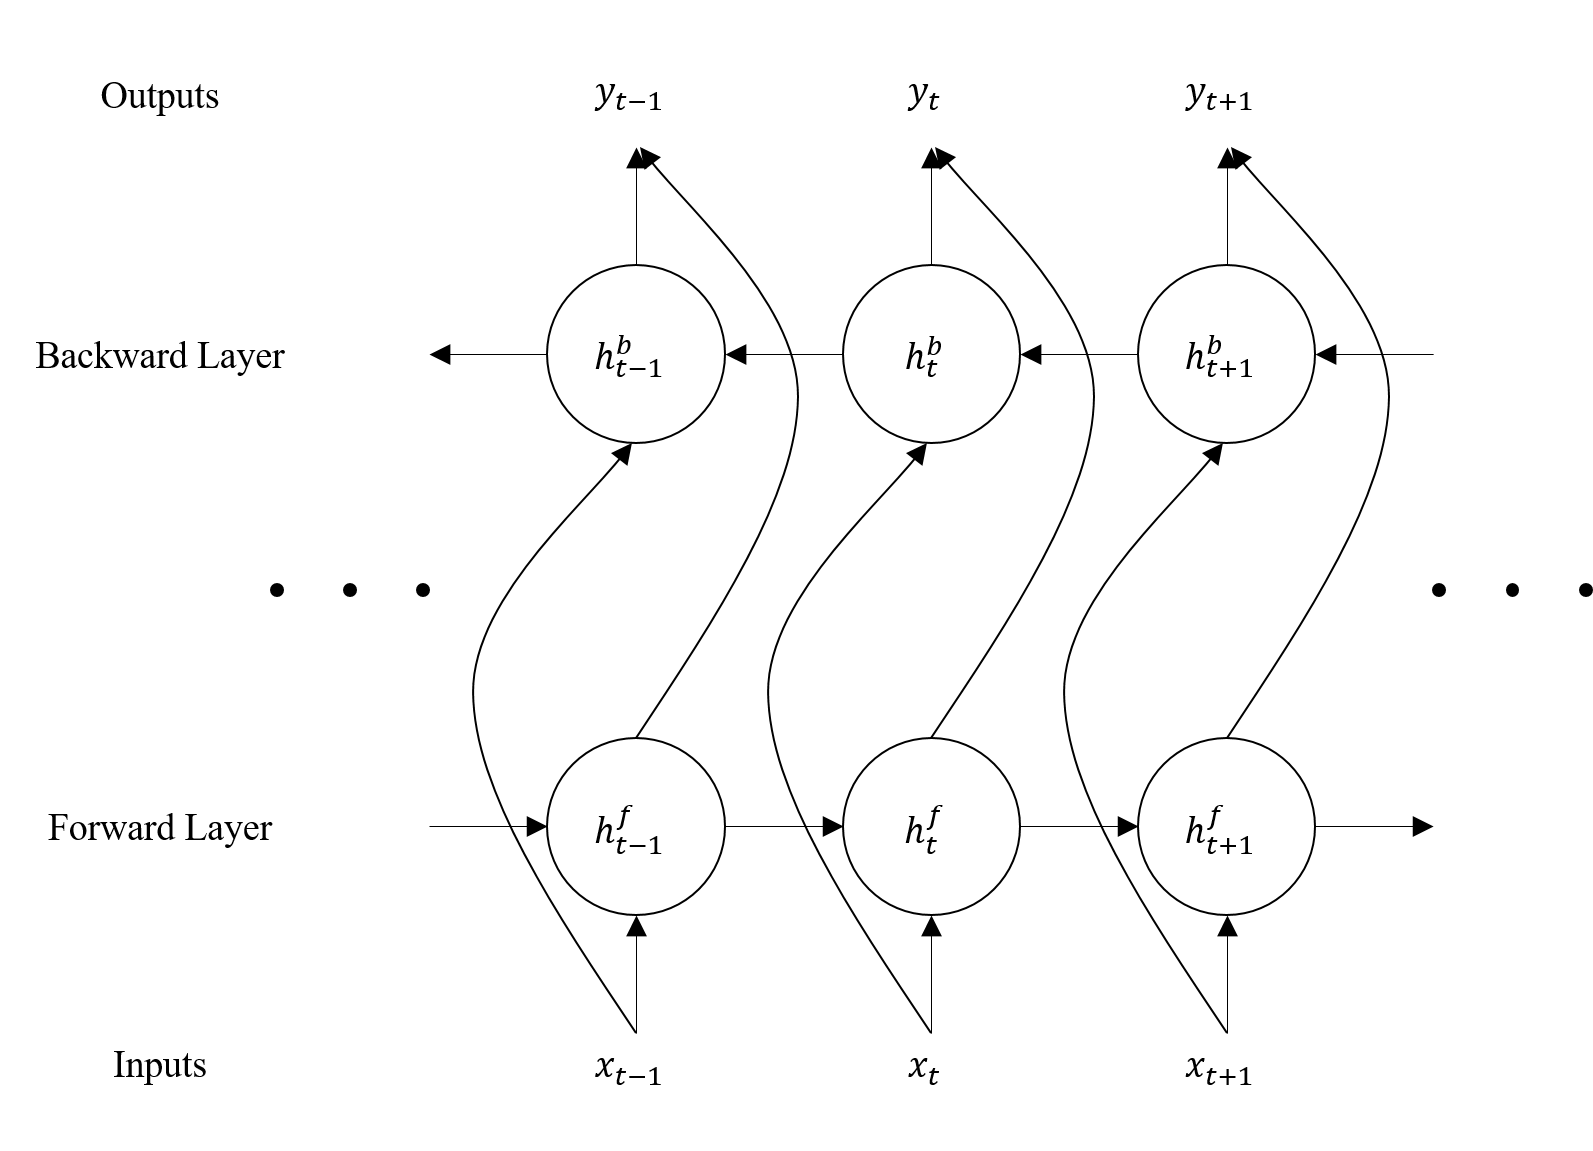
\includegraphics[width=.9\linewidth]{bidirectional}
	\label{fig:bidirectional} 	
	\caption{Bidirectional LSTM}
\end{figure}
\begin{align}
h^{f}_{t} & =\mathcal{H}\big(W_{xh^{f}}\cdot x_{t}+W_{h^{f}h^{f}}\cdot h^{f}_{t-1}+b_{h^{f}}\big)\\
h^{b}_{t} & =\mathcal{H}\big(W_{xh^{b}}\cdot x_{t}+W_{h^{b}h^{b}}\cdot h^{b}_{t-1}+b_{h^{b}}\big)\\
y_{t} & =W_{h^{f}y}\cdot h^{f}_{t}+W_{h^{b}y}\cdot h^{b}_{t}+b_{y}
\end{align}

$\mathcal{H}$ denotes the hidden layer activation function, e.g., $\tanh$ or $\sigma$. In bidirectional LSTM, upper composite function is used for $\mathcal{H}$.


\subsection{Stacked Architecture}

In deep learning, the number of layers stacked is getting large, intending to increase the non-linearity and correspondingly to improve the performance. Likewise, the multiple LSTM layers can be stacked as well \cite{dyer2015transition}, enabling more complex representation and higher performance. In stacked Bi-LSTM, total 3 LSTM layers are stacked in the series. 


And stacked bidirectional LSTM comes from the idea that the deeper networks, the better the performance of the networks as the complexity of networks increases. 


\subsection{Attention layer}

\textit{Attention} is powerful module nowadays and mostly improves performance of neural network. Originally neural networks treats information equally. But, using attention layer, neural networks can be ATTENDED what it should be examined closely. At the first time, attention is utilized at natural language processing area for improving translation performance\cite{luong2015effective}. But nowadays, attention layer is employed in many areas to improve the performance of the networks. For example, Jaderbeg \textit{et al.}\cite{jaderberg2015spatial} introduced the attention layer to let the neural networks attend to spatial information. In addition, attention is even utilized to pose estimation and optimization\cite{parisotto2018global}, detection\cite{zhu2018towards}, and video captioning\cite{xu2017learning} 

To precisely estimate the Robot’s pose and landmarks’ position, it is important for the network to distinguish which is more meaningful information and which is less \textcolor{green}{for preventing} to focus on less significant information. So, we add the two different types of attention modules \cite{luong2015effective} which extract something more important and related to the task information \textcolor{green}{by making the network to focus on different part of input sequence}. \textcolor{green}{The first attention modules placed between the input LSTM layers and the second LSTM layer are called “Spatial attention modules“. The spatial attention modules are represented as blue blocks in Fig. 2.} These attention modules can judge \textcolor{green}{which sensor has more spatial information.} The second attention \textcolor{red}{modules} corresponding to the red blocks in Fig. 2 \textcolor{red}{are} the \textcolor{green}{"Temporal attention modules". These temporal attention modules can determine which time stamp has more useful information about time,} allowing the network to attend that time stamp more.  

\subsection{Training loss}

 Unlike existing RO-SLAM methods that localize a robot by probability-based approach or filtering method like Kalman filter, etc., our approach localize  robot's position by letting the networks be trained by distance data and ground truth of the robot's position. We express the problem statement for the localization of the robot using range measurements. The training input data set is formulated as follows: 
\begin{equation}
%$L = \left\{(X_t, Y_t)\right \}$ 
L = {(X_t, Y_t)} 
\end{equation}
where $X_t = \left\{(l_1, l_2... , l_m)_t, m = 1,...,M \right \}$ denotes input range data from range sensors and $M$ is the number of UWB sensors at time $t$. Ground truth of the robot's 2D position is denoted as $Y_t = \left\{(x_t, y_t)\right \}$.

Let $\Theta$ be the parameters of a RNN model and assume that the trained RNN model could be expressed as conditional probability as follows:
\begin{equation}
P(Y_t|X_t) = p((x_t, y_t)|(l_1,..., l_m)_{t-T+1},(l_1,..., l_m)_{t-T+2}..., (l_1,..., l_m)_t)
\end{equation}  
where $T$ indicates sequential length of input to LSTM. Then, our final goal is to find optimal parameters $\Theta^{*}$ for localization by minimizing mean square error(MSE) of Euclidean distance between ground truth position $Y_k$ and estimated position $\hat{Y_k}$ as follows:
\begin{equation}
\Theta^{*} = \underset{\Theta}{\mathrm{argmin}} \frac{1}{N} \sum_{k=1}^N \parallel Y_k - \hat{Y_k} \parallel^{2}
\end{equation}  

\subsection{Why on three-dimensional?}
\subsubsection{2D}
\begin{equation}
(x-x_1)^2+(y-y_1)^2={d_1}^2
\end{equation}
\begin{equation}
(x-x_2)^2+(y-y_2)^2={d_2}^2
\end{equation}
\begin{equation}
(x-x_3)^2+(y-y_3)^2={d_3}^2
\end{equation}
\begin{equation}
(x-x_4)^2+(y-y_4)^2={d_4}^2
\end{equation}

\begin{equation}
2(x_2-x_1)x+2(y_2-y_1)y=({d_1}^2-{d_2}^2)-({x_1}^2-{x_2}^2)-({y_1}^2-{y_2}^2)
\end{equation}
\begin{equation}
2(x_3-x_1)x+2(y_3-y_1)y=({d_1}^2-{d_3}^2)-({x_1}^2-{x_3}^2)-({y_1}^2-{y_3}^2)
\end{equation}
\begin{equation}
2(x_4-x_1)x+2(y_4-y_1)y=({d_1}^2-{d_4}^2)-({x_1}^2-{x_4}^2)-({y_1}^2-{y_4}^2)
\end{equation}
\begin{equation}
A_{2D}X_{2D}=b_{2D}
\end{equation}

where $X_{2D}$ indicates $[x,y]^T$ and $A_{2D}$ and $b_{2D}$ are as follows: 

\begin{equation}
A_{2D} =\left[ {\begin{array}{cc}
	2(x_2-x_1) & 2(y_2-y_1)\\
	2(x_3-x_1) & 2(y_3-y_1)\\
	2(x_4-x_1) & 2(y_4-y_1)\\
	\end{array} } \right]
\end{equation}
\begin{equation}
b_{2D} = \left[ {\begin{array}{c}
	({d_1}^2-{d_2}^2)-({x_1}^2-{x_2}^2)-({y_1}^2-{y_2}^2)\\
	({d_1}^2-{d_3}^2)-({x_1}^2-{x_3}^2)-({y_1}^2-{y_3}^2)\\
	({d_1}^2-{d_4}^2)-({x_1}^2-{x_4}^2)-({y_1}^2-{y_4}^2)\\
	\end{array} } \right]
\end{equation}

\subsubsection{3D}

\begin{equation}
%\left\(\right\) 
(x-x_1)^2+(y-y_1)^2+(z-z_1)^2={d_1}^2
\end{equation}
\begin{equation}
(x-x_2)^2+(y-y_2)^2+(z-z_2)^2={d_2}^2
\end{equation}
\begin{equation}
(x-x_3)^2+(y-y_3)^2+(z-z_3)^2={d_3}^2
\end{equation}
\begin{equation}
(x-x_4)^2+(y-y_4)^2+(z-z_4)^2={d_4}^2
\end{equation}


\begin{equation}
2(x_2-x_1)x+2(y_2-y_1)y+2(z_2-z_1)z =  
({d_1}^2-{d_2}^2)-({x_1}^2-{x_2}^2)-({y_1}^2-{y_2}^2)-({z_1}^2-{z_2}^2)
\end{equation}
\begin{equation}
2(x_3-x_1)x+2(y_3-y_1)y+2(z_3-z_1)z=
({d_1}^2-{d_3}^2)-({x_1}^2-{x_3}^2)-({y_1}^2-{y_3}^2)-({z_1}^2-{z_3}^2)
\end{equation}
\begin{equation}
\substack{
	2(x_4-x_1)x+2(y_4-y_1)y+2(z_4-z_1)z=
	({d_1}^2-{d_4}^2)-({x_1}^2-{x_4}^2)-({y_1}^2-{y_4}^2)-({z_1}^2-{z_4}^2)
}
\end{equation}
\begin{equation}
A_{3D}X_{3D}=b_{3D}
\end{equation}

where $X_{3D}$ indicates $[x,y,z]^T$ and $A_{3D}$ and $b_{3D}$ are as follows: 

\begin{equation}
A_{3D} =\left[ {\begin{array}{ccc}
	2(x_2-x_1) & 2(y_2-y_1) & 2(z_2-z_1)\\
	2(x_3-x_1) & 2(y_3-y_1) & 2(z_3-z_1)\\
	2(x_4-x_1) & 2(y_4-y_1) & 2(z_4-z_1)\\
	\end{array} } \right]
\end{equation}
\begin{equation}
b_{3D} = \left[ {\begin{array}{c}
	\substack{
		({d_1}^2-{d_2}^2)-({x_1}^2-{x_2}^2)-({y_1}^2-{y_2}^2)-({z_1}^2-{z_2}^2)\\
		({d_1}^2-{d_3}^2)-({x_1}^2-{x_3}^2)-({y_1}^2-{y_3}^2)-({z_1}^2-{z_3}^2)\\
		({d_1}^2-{d_4}^2)-({x_1}^2-{x_4}^2)-({y_1}^2-{y_4}^2)-({z_1}^2-{z_4}^2)\\
	}
	\end{array} } \right]
\end{equation}

Unlike the case of 2D, $A_{3D}$ consists of $z$ components on the third column. Let $a_{3D}^{ij}$ be the $i^{th}$ row and $j^{th}$ component of $A_{3D}$. In ideal case the anchor nodes are placed to square position with equal height, then $a_{3D}^{12}$, $a_{3D}^{31}$, and elements of the third colums are equal to zero. This cause the rank dificiency, however that terms could not be the zero even though the anchor nodes are placed carefully. in real-world, it is hard to put the anchor nodes with exactly same position. As a result, $z_1\approx z_2\approx z_3\approx z_4$ $A_{3D}$  



\section{Experiments}
\subsection{Experimental environment}

\begin{figure*}[h]
	\centering
	\begin{subfigure}[b]{.25\textwidth}
		\centering
		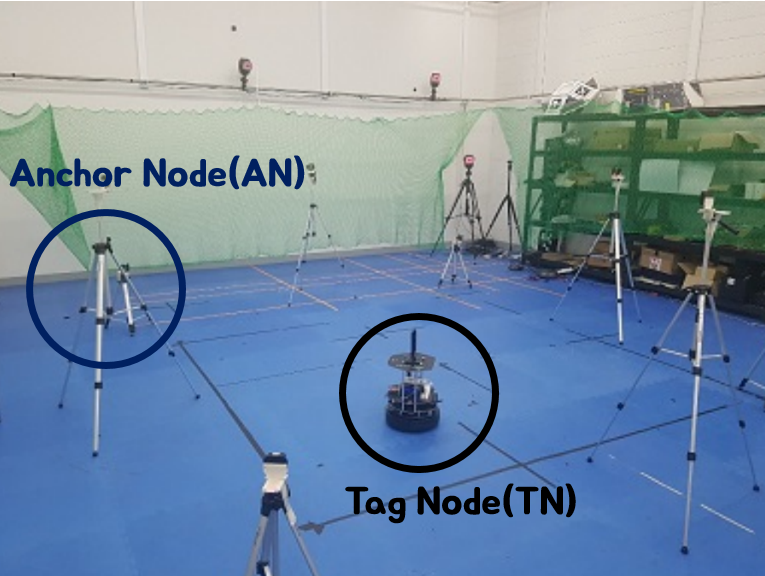
\includegraphics[width=.9\textwidth]{anchor_tag_nodes}
		\label{fig:dataset} 	
		\caption{}
	\end{subfigure}%
	\begin{subfigure}[b]{.25\textwidth}
		\centering
		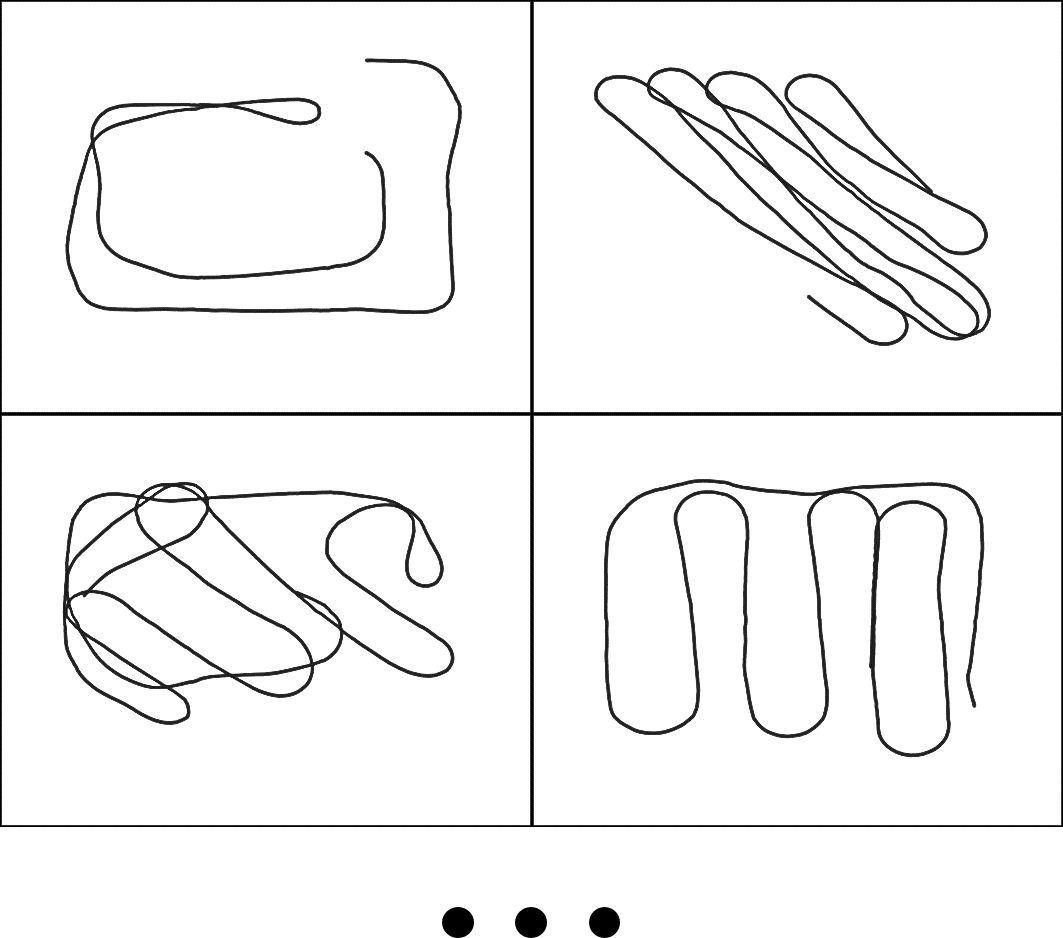
\includegraphics[width=0.9\textwidth]{paths}
		\label{fig:nodes} 	
		\caption{}
	\end{subfigure}%
	\begin{subfigure}[b]{.5\textwidth}
		\centering
		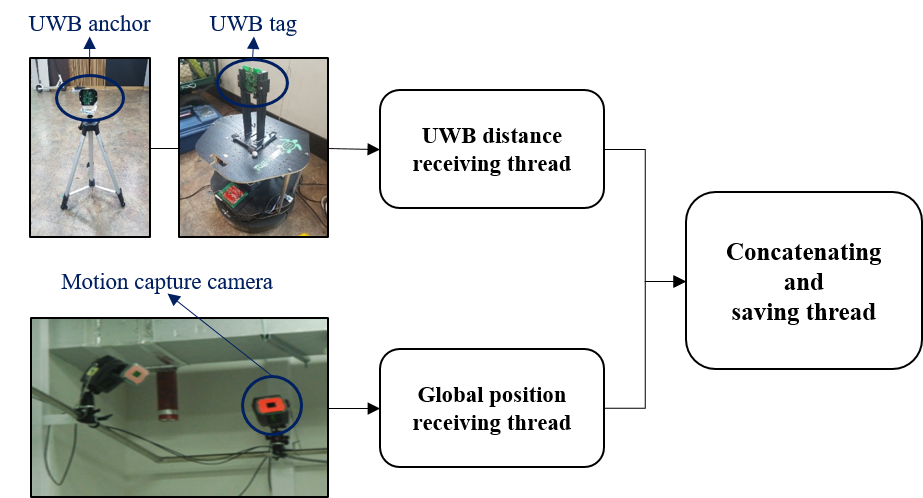
\includegraphics[width=0.9\textwidth]{dataset_process}
		\label{fig:trajectories} 	
		\caption{}
	\end{subfigure}
	\caption{Figures from experiment (a)The anchor and tag nodes (b)Four examples of the trajectory (c) the process that makes dataset}
	\label{fig:experiment}
\end{figure*}
Our experimental system consists of a UWB(ultra wideband) sensor tag and eight anchors that have a UWB transceiver, the motion capture system with 12 cameras, a mobile robot and a small form-factor computer.

UWB sensor anchors are attached to landmarks. These become the end points of the range measurements. The anchor nodes transmit the UWB signal. A UWB sensor tag is attached to a robot. It becomes the opposite side end point of the measurements. The tag node receives the signal and measures the range between two devices. Each UWB transceiver, DW1000 UWB-chip made by Decawave, supports 6 RF bands from 3.5 GHz to 6.5 GHz. It measures in centimeter-level accuracy. Fig. \ref{fig:experiment}(a) shows anchor and tag nodes.

We inference the position of a robot with our network. To train the network and test the results, the ground truths are needed. We get the ground truth by using the motion capture system. The system is Eagle Digital Realtime system of motion analysis corporation that operates with the principle of stereo pattern recognition that is a kind of photogrammetry based on the epipolar geometry and the triangulation methodology. We attach four markers to a robot. The system gives us the location of these markers and has < 1mm accuracy.

A mobile robot used in experiment is iClebo Kobuki from Yujinrobot that has 70 cm/s maximum velocity.The small form-factor computer is a gigabyte Ultra compact PC. Deep learning framework used for our network is pytorch 0.4.0 on python 3.6. The network inferences on the same setting.

The UWB tag is attached to mobile robot that has a small compact computer. The UWB anchors are attached to stands that have two different heights. The anchors are positioned randomly in the square space. As you can see in Fig. \ref{fig:experiment}(b), a mobile robot manually goes on various random trajectories by experimenters.

During the robot is going on, the data is saved in the computer. The distance data used for input data is measured by the UWB sensors. The global position data used for ground truth is measured by the motion capture system. These two kinds of data are paired in a dataset. The computer receives these two kinds of data respectively and syncronizes these by time. To synchronize, we make an independent thread that concatenates and saves these data at the same time. The data is saved at 20Hz frequency. Each trajectory becomes one dataset. All the trajectories are different. Fig. \ref{fig:experiment}(c) shows this process. After collecting whole datasets, we separate the entire dataset to two types, some are the training datasets and others are test datasets.

\subsection{Data syncronization for Train/Test data}
\subsection{Training the Networks}


\section{Results}

\textcolor{green}{To verify our proposal that RNNs can estimate the robot's position through varying range data, we trained our RNN-based multimodal architecture. Plus, to compare to previous traditional SLAM algorithm, we also estimate robot's position by particle filter(PF) based algorithm.}

As illustrated in Experiment session, train data are our own data gathered by UWB sensors and motion capture camera, so neural networks take range-only measurements as input and output robot's position. Ground truth data is robot's position measured by eagle eye motion capturer, whose error is in mm units. The results of trajectory prediction are shown in Fig. \ref{fig:trajectory} and Root-Mean-Squared Error (RMSE) are shown in Table \ref{table:RMSE_table}. Note that out experiment is conducted on mobile robot, so we can pre-estimates that z position of robot is almost similar while robot is running. 

We set two test trajectory cases: an square path and zigzag path. an The results shows that it has better performance than established probabilistic-based approach. In both cases, performance of our networks  is better that of particle filter. RMSE of our networks in test1 is 3.928cm and 4.119cm in test2.

We also verified effectiveness of attention layer. It was confirmed that the performance of the networks with the attention layer is improved compared to the networks without the attention layer.

\begin{table}[h]
	\begin{tabular}{lllcc}
		\hline
		\multicolumn{5}{c}{The results of RMSE{[}cm{]}}                                                                          \\ \hline
		\multicolumn{3}{c|}{Model}                                        & \multicolumn{1}{c|}{Test1}          & Test2          \\ \hline
		\multicolumn{3}{l|}{Particle Filter-based w/o pre-estimates of z} & \multicolumn{1}{c|}{11.253}         & 9.195          \\
		\multicolumn{3}{l|}{Particle Filter-based}                        & \multicolumn{1}{c|}{5.525}          & 5.258          \\
		\multicolumn{3}{l|}{Multimodal(Ours)}                                   & \multicolumn{1}{c|}{4.225}          & 4.311          \\
		\multicolumn{3}{l|}{Multimodal(Ours) + attention}                       & \multicolumn{1}{c|}{\textbf{3.928}} & \textbf{4.119}
	\end{tabular}
	\caption{Root mean squared error of each case}
	\label{table:RMSE_table}
\end{table}



\section{Conclusion}

In this paper, we proposed a novel approach to range-only SLAM using multimodal-based RNN models and tested our architectures in two test data.

Using deep learning, our structure directly learns the end-to-end mapping between distance data and robot position. The multimodal bidirectional stacked LSTM structure exhibits the precise estimates of robot positions. We set two test trajectory cases: an square path and zigzag path. an The results shows that it has better performance than established probabilistic-based approach. In both cases, performance of our networks  is better that of particle filter. RMSE of our networks in test1 is 3.928cm and 4.119cm in test2. Therefore, we could check the possibility that our multimodal LSTM-based structure can substitute traditional algorithms

As a future work, because we conducted on just localization, this approach may not be operated when locations of sensors are changed. Therefore, the proposed method needs to be revised for precise estimates even though locations of anchors are changed. 

\appendices

Appendixes, if needed, appear before the acknowledgment.

\section*{Acknowledgment}

The preferred spelling of the word ``acknowledgment'' in American English is 
without an ``e'' after the ``g.'' Use the singular heading even if you have 
many acknowledgments. Avoid expressions such as ``One of us (S.B.A.) would 
like to thank $\ldots$ .'' Instead, write ``F. A. Author thanks $\ldots$ .'' In most 
cases, sponsor and financial support acknowledgments are placed in the 
unnumbered footnote on the first page, not here.

\section*{References and Footnotes}

\subsection{References}
References need not be cited in text. When they are, they appear on the 
line, in square brackets, inside the punctuation. Multiple references are 
each numbered with separate brackets. When citing a section in a book, 
please give the relevant page numbers. In text, refer simply to the 
reference number. Do not use ``Ref.'' or ``reference'' except at the 
beginning of a sentence: ``Reference \cite{b3} shows $\ldots$ .'' Please do not use 
automatic endnotes in \emph{Word}, rather, type the reference list at the end of the 
paper using the ``References'' style.

Reference numbers are set flush left and form a column of their own, hanging 
out beyond the body of the reference. The reference numbers are on the line, 
enclosed in square brackets. In all references, the given name of the author 
or editor is abbreviated to the initial only and precedes the last name. Use 
them all; use \emph{et al.} only if names are not given. Use commas around Jr., 
Sr., and III in names. Abbreviate conference titles. When citing IEEE 
transactions, provide the issue number, page range, volume number, year, 
and/or month if available. When referencing a patent, provide the day and 
the month of issue, or application. References may not include all 
information; please obtain and include relevant information. Do not combine 
references. There must be only one reference with each number. If there is a 
URL included with the print reference, it can be included at the end of the 
reference. 

Other than books, capitalize only the first word in a paper title, except 
for proper nouns and element symbols. For papers published in translation 
journals, please give the English citation first, followed by the original 
foreign-language citation See the end of this document for formats and 
examples of common references. For a complete discussion of references and 
their formats, see the IEEE style manual at
\underline{http://www.ieee.org/authortools}.

\subsection{Footnotes}
Number footnotes separately in superscript numbers.\footnote{It is recommended that footnotes be avoided (except for 
the unnumbered footnote with the receipt date on the first page). Instead, 
try to integrate the footnote information into the text.} Place the actual 
footnote at the bottom of the column in which it is cited; do not put 
footnotes in the reference list (endnotes). Use letters for table footnotes 
(see Table \ref{table}).

\section{Submitting Your Paper for Review}

\subsection{Final Stage}
When you submit your final version (after your paper has been accepted), 
print it in two-column format, including figures and tables. You must also 
send your final manuscript on a disk, via e-mail, or through a Web 
manuscript submission system as directed by the society contact. You may use 
\emph{Zip} for large files, or compress files using \emph{Compress, Pkzip, Stuffit,} or \emph{Gzip.} 

Also, send a sheet of paper or PDF with complete contact information for all 
authors. Include full mailing addresses, telephone numbers, fax numbers, and 
e-mail addresses. This information will be used to send each author a 
complimentary copy of the journal in which the paper appears. In addition, 
designate one author as the ``corresponding author.'' This is the author to 
whom proofs of the paper will be sent. Proofs are sent to the corresponding 
author only.

\subsection{Review Stage Using ScholarOne\textregistered\ Manuscripts}
Contributions to the Transactions, Journals, and Letters may be submitted 
electronically on IEEE's on-line manuscript submission and peer-review 
system, ScholarOne\textregistered\ Manuscripts. You can get a listing of the 
publications that participate in ScholarOne at 
\underline{http://www.ieee.org/publications\_standards/publications/}\break\underline{authors/authors\_submission.html}.
First check if you have an existing account. If there is none, please create 
a new account. After logging in, go to your Author Center and click ``Submit 
First Draft of a New Manuscript.'' 

Along with other information, you will be asked to select the subject from a 
pull-down list. Depending on the journal, there are various steps to the 
submission process; you must complete all steps for a complete submission. 
At the end of each step you must click ``Save and Continue''; just uploading 
the paper is not sufficient. After the last step, you should see a 
confirmation that the submission is complete. You should also receive an 
e-mail confirmation. For inquiries regarding the submission of your paper on 
ScholarOne Manuscripts, please contact oprs-support@ieee.org or call +1 732 
465 5861.

ScholarOne Manuscripts will accept files for review in various formats. 
Please check the guidelines of the specific journal for which you plan to 
submit.

You will be asked to file an electronic copyright form immediately upon 
completing the submission process (authors are responsible for obtaining any 
security clearances). Failure to submit the electronic copyright could 
result in publishing delays later. You will also have the opportunity to 
designate your article as ``open access'' if you agree to pay the IEEE open 
access fee. 

\subsection{Final Stage Using ScholarOne Manuscripts}
Upon acceptance, you will receive an email with specific instructions 
regarding the submission of your final files. To avoid any delays in 
publication, please be sure to follow these instructions. Most journals 
require that final submissions be uploaded through ScholarOne Manuscripts, 
although some may still accept final submissions via email. Final 
submissions should include source files of your accepted manuscript, high 
quality graphic files, and a formatted pdf file. If you have any questions 
regarding the final submission process, please contact the administrative 
contact for the journal. 

In addition to this, upload a file with complete contact information for all 
authors. Include full mailing addresses, telephone numbers, fax numbers, and 
e-mail addresses. Designate the author who submitted the manuscript on 
ScholarOne Manuscripts as the ``corresponding author.'' This is the only 
author to whom proofs of the paper will be sent. 

\subsection{Copyright Form}
Authors must submit an electronic IEEE Copyright Form (eCF) upon submitting 
their final manuscript files. You can access the eCF system through your 
manuscript submission system or through the Author Gateway. You are 
responsible for obtaining any necessary approvals and/or security 
clearances. For additional information on intellectual property rights, 
visit the IEEE Intellectual Property Rights department web page at 
\underline{http://www.ieee.org/publications\_standards/publications/}\break\underline{rights/index.html}. 

\section{IEEE Publishing Policy}
The general IEEE policy requires that authors should only submit original 
work that has neither appeared elsewhere for publication, nor is under 
review for another refereed publication. The submitting author must disclose 
all prior publication(s) and current submissions when submitting a 
manuscript. Do not publish ``preliminary'' data or results. The submitting 
author is responsible for obtaining agreement of all coauthors and any 
consent required from employers or sponsors before submitting an article. 
The IEEE Access Department strongly discourages courtesy 
authorship; it is the obligation of the authors to cite only relevant prior 
work.

The IEEE Access Department does not publish conference 
records or proceedings, but can publish articles related to conferences that 
have undergone rigorous peer review. Minimally, two reviews are required for 
every article submitted for peer review.

\section{Publication Principles}
The two types of contents of that are published are; 1) peer-reviewed and 2) 
archival. The Access Department publishes scholarly 
articles of archival value as well as tutorial expositions and critical 
reviews of classical subjects and topics of current interest. 

Authors should consider the following points:

\begin{enumerate}
\item Technical papers submitted for publication must advance the state of knowledge and must cite relevant prior work. 
\item The length of a submitted paper should be commensurate with the importance, or appropriate to the complexity, of the work. For example, an obvious extension of previously published work might not be appropriate for publication or might be adequately treated in just a few pages.
\item Authors must convince both peer reviewers and the editors of the scientific and technical merit of a paper; the standards of proof are higher when extraordinary or unexpected results are reported. 
\item Because replication is required for scientific progress, papers submitted for publication must provide sufficient information to allow readers to perform similar experiments or calculations and 
use the reported results. Although not everything need be disclosed, a paper 
must contain new, useable, and fully described information. For example, a 
specimen's chemical composition need not be reported if the main purpose of 
a paper is to introduce a new measurement technique. Authors should expect 
to be challenged by reviewers if the results are not supported by adequate 
data and critical details.
\item Papers that describe ongoing work or announce the latest technical achievement, which are suitable for presentation at a professional conference, may not be appropriate for publication.
\end{enumerate}

\bibliographystyle{IEEEtran}
% argument is your BibTeX string definitions and bibliography database(s)
\bibliography{./Access_RObib}


\begin{IEEEbiography}[{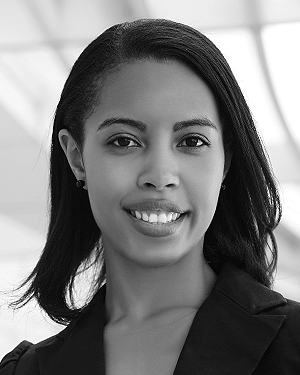
\includegraphics[width=1in,height=1.25in,clip,keepaspectratio]{a1.png}}]{First A. Author} (M'76--SM'81--F'87) and all authors may include 
biographies. Biographies are often not included in conference-related
papers. This author became a Member (M) of IEEE in 1976, a Senior
Member (SM) in 1981, and a Fellow (F) in 1987. The first paragraph may
contain a place and/or date of birth (list place, then date). Next,
the author's educational background is listed. The degrees should be
listed with type of degree in what field, which institution, city,
state, and country, and year the degree was earned. The author's major
field of study should be lower-cased. 

The second paragraph uses the pronoun of the person (he or she) and not the 
author's last name. It lists military and work experience, including summer 
and fellowship jobs. Job titles are capitalized. The current job must have a 
location; previous positions may be listed 
without one. Information concerning previous publications may be included. 
Try not to list more than three books or published articles. The format for 
listing publishers of a book within the biography is: title of book 
(publisher name, year) similar to a reference. Current and previous research 
interests end the paragraph. The third paragraph begins with the author's 
title and last name (e.g., Dr.\ Smith, Prof.\ Jones, Mr.\ Kajor, Ms.\ Hunter). 
List any memberships in professional societies other than the IEEE. Finally, 
list any awards and work for IEEE committees and publications. If a 
photograph is provided, it should be of good quality, and 
professional-looking. Following are two examples of an author's biography.
\end{IEEEbiography}

\begin{IEEEbiography}[{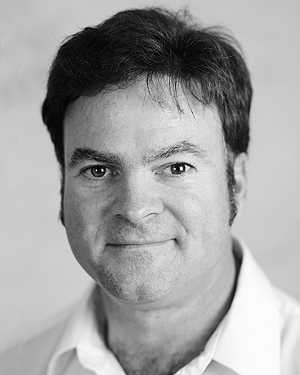
\includegraphics[width=1in,height=1.25in,clip,keepaspectratio]{a2.png}}]{Second B. Author} was born in Greenwich Village, New York, NY, USA in 
1977. He received the B.S. and M.S. degrees in aerospace engineering from 
the University of Virginia, Charlottesville, in 2001 and the Ph.D. degree in 
mechanical engineering from Drexel University, Philadelphia, PA, in 2008.

From 2001 to 2004, he was a Research Assistant with the Princeton Plasma 
Physics Laboratory. Since 2009, he has been an Assistant Professor with the 
Mechanical Engineering Department, Texas A{\&}M University, College Station. 
He is the author of three books, more than 150 articles, and more than 70 
inventions. His research interests include high-pressure and high-density 
nonthermal plasma discharge processes and applications, microscale plasma 
discharges, discharges in liquids, spectroscopic diagnostics, plasma 
propulsion, and innovation plasma applications. He is an Associate Editor of 
the journal \emph{Earth, Moon, Planets}, and holds two patents. 

Dr. Author was a recipient of the International Association of Geomagnetism 
and Aeronomy Young Scientist Award for Excellence in 2008, and the IEEE 
Electromagnetic Compatibility Society Best Symposium Paper Award in 2011. 
\end{IEEEbiography}

\begin{IEEEbiography}[{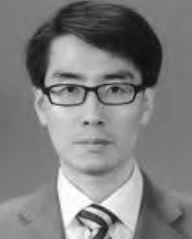
\includegraphics[width=1in,height=1.25in,clip,keepaspectratio]{a3.png}}]{Third C. Author, Jr.} (M'87) received the B.S. degree in mechanical 
engineering from National Chung Cheng University, Chiayi, Taiwan, in 2004 
and the M.S. degree in mechanical engineering from National Tsing Hua 
University, Hsinchu, Taiwan, in 2006. He is currently pursuing the Ph.D. 
degree in mechanical engineering at Texas A{\&}M University, College 
Station, TX, USA.

From 2008 to 2009, he was a Research Assistant with the Institute of 
Physics, Academia Sinica, Tapei, Taiwan. His research interest includes the 
development of surface processing and biological/medical treatment 
techniques using nonthermal atmospheric pressure plasmas, fundamental study 
of plasma sources, and fabrication of micro- or nanostructured surfaces. 

Mr. Author's awards and honors include the Frew Fellowship (Australian 
Academy of Science), the I. I. Rabi Prize (APS), the European Frequency and 
Time Forum Award, the Carl Zeiss Research Award, the William F. Meggers 
Award and the Adolph Lomb Medal (OSA).
\end{IEEEbiography}

\EOD

\end{document}
